% Options for packages loaded elsewhere
\PassOptionsToPackage{unicode}{hyperref}
\PassOptionsToPackage{hyphens}{url}
%
\documentclass[
  11pt,
  ignorenonframetext,
]{beamer}
\usepackage{pgfpages}
\setbeamertemplate{caption}[numbered]
\setbeamertemplate{caption label separator}{: }
\setbeamercolor{caption name}{fg=normal text.fg}
\beamertemplatenavigationsymbolsempty
% Prevent slide breaks in the middle of a paragraph
\widowpenalties 1 10000
\raggedbottom
\setbeamertemplate{part page}{
  \centering
  \begin{beamercolorbox}[sep=16pt,center]{part title}
    \usebeamerfont{part title}\insertpart\par
  \end{beamercolorbox}
}
\setbeamertemplate{section page}{
  \centering
  \begin{beamercolorbox}[sep=12pt,center]{part title}
    \usebeamerfont{section title}\insertsection\par
  \end{beamercolorbox}
}
\setbeamertemplate{subsection page}{
  \centering
  \begin{beamercolorbox}[sep=8pt,center]{part title}
    \usebeamerfont{subsection title}\insertsubsection\par
  \end{beamercolorbox}
}
\AtBeginPart{
  \frame{\partpage}
}
\AtBeginSection{
  \ifbibliography
  \else
    \frame{\sectionpage}
  \fi
}
\AtBeginSubsection{
  \frame{\subsectionpage}
}
\usepackage{amsmath,amssymb}
\usepackage{lmodern}
\usepackage{iftex}
\ifPDFTeX
  \usepackage[T1]{fontenc}
  \usepackage[utf8]{inputenc}
  \usepackage{textcomp} % provide euro and other symbols
\else % if luatex or xetex
  \usepackage{unicode-math}
  \defaultfontfeatures{Scale=MatchLowercase}
  \defaultfontfeatures[\rmfamily]{Ligatures=TeX,Scale=1}
\fi
\usetheme[]{metropolis}
% Use upquote if available, for straight quotes in verbatim environments
\IfFileExists{upquote.sty}{\usepackage{upquote}}{}
\IfFileExists{microtype.sty}{% use microtype if available
  \usepackage[]{microtype}
  \UseMicrotypeSet[protrusion]{basicmath} % disable protrusion for tt fonts
}{}
\makeatletter
\@ifundefined{KOMAClassName}{% if non-KOMA class
  \IfFileExists{parskip.sty}{%
    \usepackage{parskip}
  }{% else
    \setlength{\parindent}{0pt}
    \setlength{\parskip}{6pt plus 2pt minus 1pt}}
}{% if KOMA class
  \KOMAoptions{parskip=half}}
\makeatother
\usepackage{xcolor}
\newif\ifbibliography
\usepackage{graphicx}
\makeatletter
\def\maxwidth{\ifdim\Gin@nat@width>\linewidth\linewidth\else\Gin@nat@width\fi}
\def\maxheight{\ifdim\Gin@nat@height>\textheight\textheight\else\Gin@nat@height\fi}
\makeatother
% Scale images if necessary, so that they will not overflow the page
% margins by default, and it is still possible to overwrite the defaults
% using explicit options in \includegraphics[width, height, ...]{}
\setkeys{Gin}{width=\maxwidth,height=\maxheight,keepaspectratio}
% Set default figure placement to htbp
\makeatletter
\def\fps@figure{htbp}
\makeatother
\setlength{\emergencystretch}{3em} % prevent overfull lines
\providecommand{\tightlist}{%
  \setlength{\itemsep}{0pt}\setlength{\parskip}{0pt}}
\setcounter{secnumdepth}{-\maxdimen} % remove section numbering
\ifLuaTeX
  \usepackage{selnolig}  % disable illegal ligatures
\fi
\IfFileExists{bookmark.sty}{\usepackage{bookmark}}{\usepackage{hyperref}}
\IfFileExists{xurl.sty}{\usepackage{xurl}}{} % add URL line breaks if available
\urlstyle{same} % disable monospaced font for URLs
\hypersetup{
  pdftitle={Conceptos básicos de estadística},
  pdfauthor={Gerardo Martín},
  hidelinks,
  pdfcreator={LaTeX via pandoc}}

\title{Conceptos básicos de estadística}
\subtitle{Clasificación de variables}
\author{Gerardo Martín}
\date{2022-06-29}

\begin{document}
\frame{\titlepage}

\begin{frame}{Por su naturaleza matemática}
\protect\hypertarget{por-su-naturaleza-matemuxe1tica}{}
\begin{itemize}
\item
  Continuas
\item
  Discretas
\item
  Categoricas
\item
  Ordinales
\end{itemize}
\end{frame}

\begin{frame}{Por su papel en el estudio}
\protect\hypertarget{por-su-papel-en-el-estudio}{}
\begin{itemize}
\item
  Independientes
\item
  Dependientes
\end{itemize}
\end{frame}

\hypertarget{variables-independientes}{%
\section{Variables independientes}\label{variables-independientes}}

\begin{frame}{¿Qué son?}
\protect\hypertarget{quuxe9-son}{}
Procesos o fuerzas externas que afectan nuestro sistema de estudio

Sistema de estudio \emph{no las afectan}

Generalmente hay más de una
\end{frame}

\begin{frame}{¿Qué son?}
\protect\hypertarget{quuxe9-son-1}{}
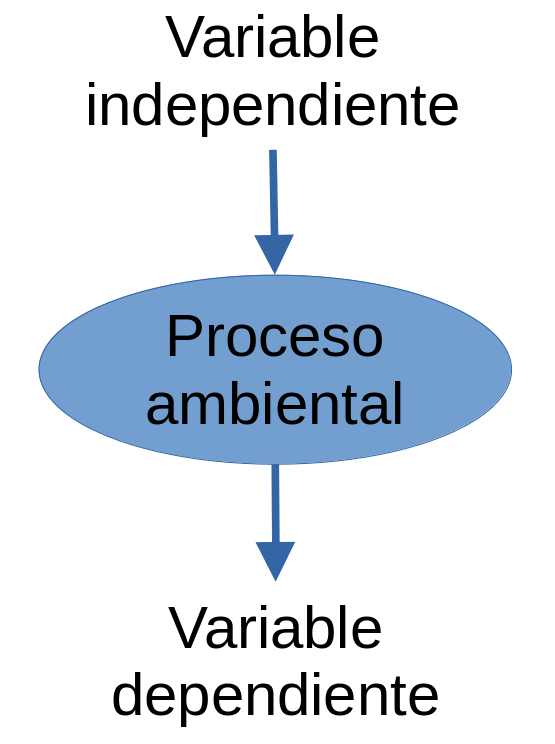
\includegraphics{Figuras-variables/Tipos-variables.png}
\end{frame}

\begin{frame}{Ejemplo}
\protect\hypertarget{ejemplo}{}
La visión es posible gracias a la luz

La visión no crea la luz
\end{frame}

\begin{frame}{Ejemplo}
\protect\hypertarget{ejemplo-1}{}
Temperatura afecta desarrollo de plántulas

Plántulas no afectan condiciones de temperatura
\end{frame}

\hypertarget{variables-dependientes}{%
\section{Variables dependientes}\label{variables-dependientes}}

\begin{frame}{¿Qué es?}
\protect\hypertarget{quuxe9-es}{}
Proceso principal de estudio

Es afectado o generado por las variables independientes

Generalmente sólo hay una
\end{frame}

\begin{frame}{Ejemplos}
\protect\hypertarget{ejemplos}{}
En un estudio de actitudes sociales a los proyectos de conservación:

\begin{itemize}
\item
  \textbf{Variable dependiente}: Actitud o percepción de los proyectos
\item
  \textbf{Variable(s) independiente(s)}: Condición socioeconómica del/la
  entrevistadx, edad
\end{itemize}
\end{frame}

\begin{frame}{Ejemplos}
\protect\hypertarget{ejemplos-1}{}
En un estudio del efecto del fuego sobre germinación de semillas

\begin{itemize}
\item
  \textbf{Variable dependiente}: Porcentaje de germinación
\item
  \textbf{Variable independiente}: Intensidad del fuego, temporada de
  ocurrencia del fuego
\end{itemize}
\end{frame}

\begin{frame}{Ejemplos}
\protect\hypertarget{ejemplos-2}{}
En un estudio de la temperatura en microhábitats

\begin{itemize}
\item
  \textbf{Variable dependiente}: Temperatura a nivel del suelo
\item
  \textbf{Variables independientes}: Temperatura del aire, radiación
  solar, cobertura arbórea, velocidad del viento
\end{itemize}
\end{frame}

\end{document}
